\documentclass{article}
\usepackage{graphicx}
\usepackage{float}
\usepackage{amsmath}
\usepackage{amsfonts}
\usepackage{amssymb}
\usepackage{hyperref}
\usepackage{esint}
\usepackage[utf8]{inputenc}
\usepackage[a4paper, portrait, margin=0.75in]{geometry}
\setlength\parindent{0pt}
\usepackage[italian]{babel}
\usepackage{tikz}
\usepackage{circuitikz}





\hypersetup{
    colorlinks=true,
    linkcolor=black,
    filecolor=magenta,
    urlcolor=blue,
    pdftitle={Tecnologie internet},
    pdfpagemode=FullScreen,
}


\begin{document}
    \author{kanopo}
    \title{Economia}
    \date{2022}

    \maketitle
    \tableofcontents

    \listoffigures
    \listoftables

\section{Elementi di economia d'impresa}

ho perso il riassunto da pag 0 a pag 55
dio cane
\section{Introduzione alla gestione aziendale}
\subsection{Gestione d'impresa e attività decisionale}


\begin{itemize}
    \item L'impresa è un sistema socio tecnico aperto
    \item gli obiettivi vengono perseguiti con l'attività decisionale(migliorare produzione e soddisfazione cliente)
\end{itemize}

\begin{figure}[H]
    \centering
    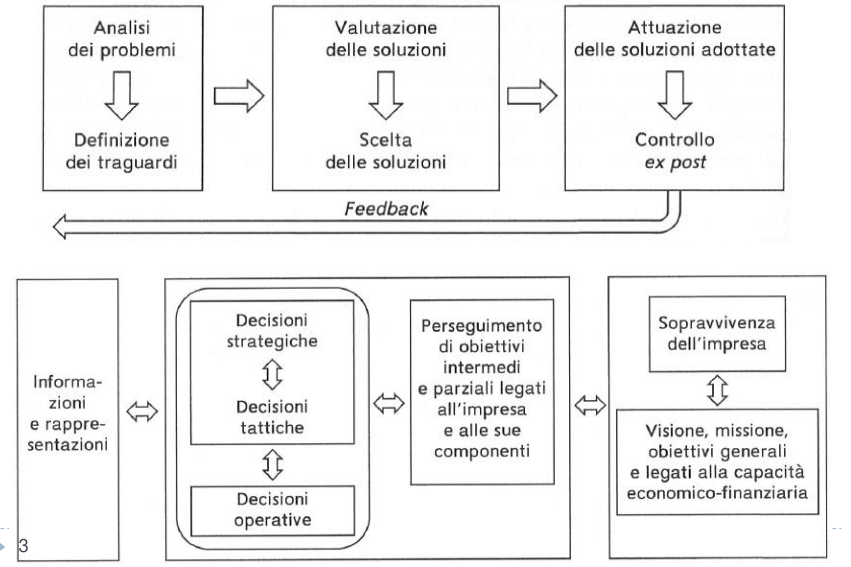
\includegraphics[width=0.7\linewidth]{1/img/Screenshot from 2022-07-03 11-30-16.png}
\end{figure}

\subsection{Criteri di scelta nelle decisioni d'impresa}


3 criteri:
\begin{itemize}
    \item efficacia: scelta e realizzazione degli obbiettivi
    \item efficienza: minimizzare le risorse
        \begin{itemize}
            \item produttività: effcienza tecnica
            \item economicità: effcienza economica
        \end{itemize}
    \item redditività
\end{itemize}

\begin{figure}[H]
    \centering
    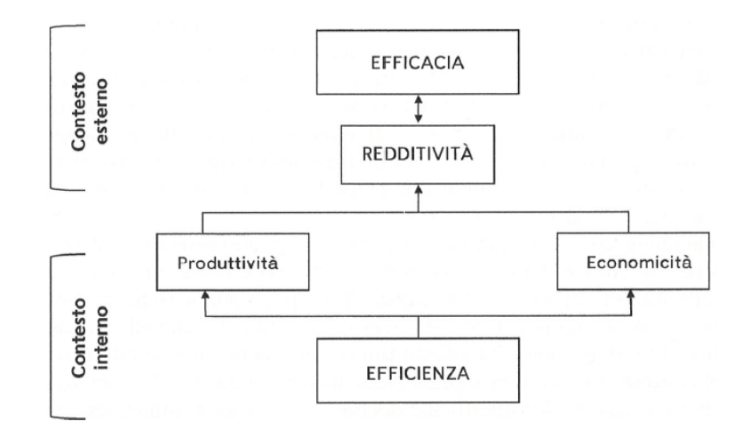
\includegraphics[width=0.5\linewidth]{1/img/Screenshot from 2022-07-03 11-35-16.png}
\end{figure}

\subsection{Incertezza e ambiguità nelle decisioni d'impresa}

\begin{figure}[H]
    \centering
    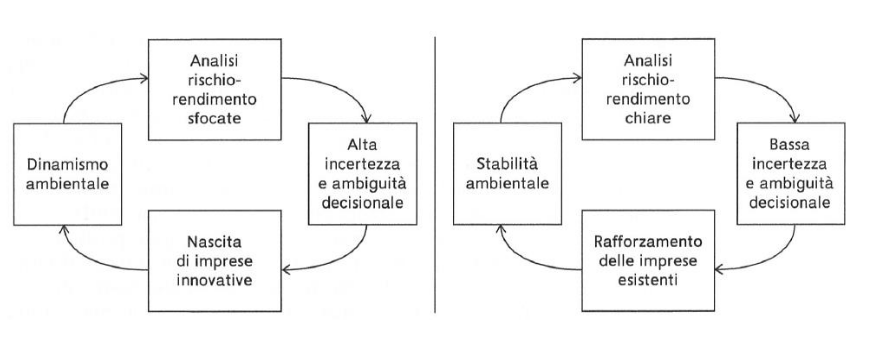
\includegraphics[width=0.7\linewidth]{1/img/Screenshot from 2022-07-03 11-36-56.png}
\end{figure}

\subsection{Le aree funzionali di gestione}

\begin{figure}[H]
    \centering
    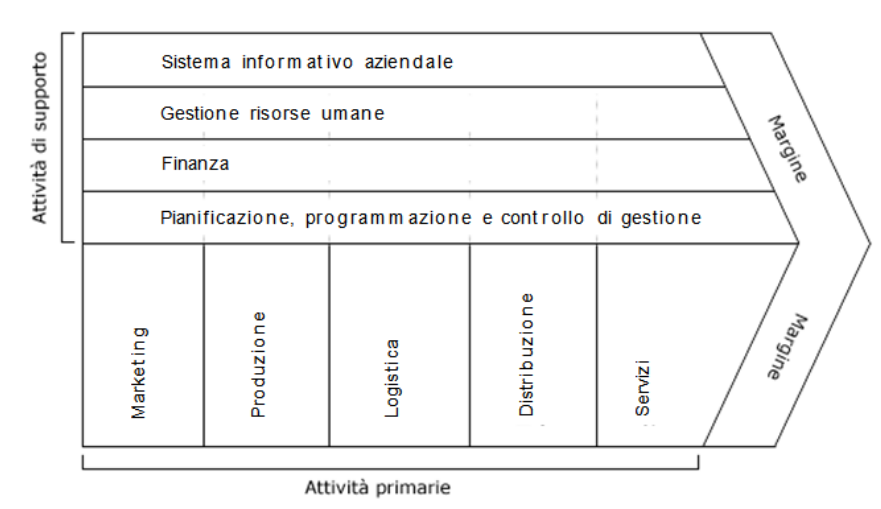
\includegraphics[width=0.7\linewidth]{1/img/Screenshot from 2022-07-03 16-14-51.png}
\end{figure}

\subsection{Marketing}
Attività volte a soddisfare le esigenze dei consumatori fornendo prodotti e servizi.

\subsection{Produzione}
Attività volte alla realizzazione di un prodotto o servizio.

Segue breve classificazione di processi produttivi:
\begin{figure}[H]
    \centering
    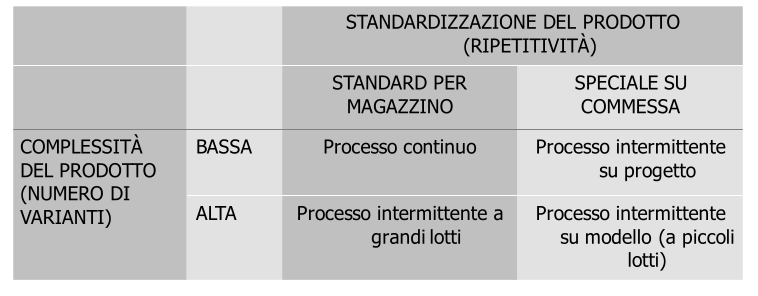
\includegraphics[width=0.5\linewidth]{1/img/Screenshot from 2022-07-04 14-59-14.png}
\end{figure}


La valutazione dell'investimento industriale richiede di considerare i seguenti aspetti:
\begin{itemize}
    \item domanda del mercato
    \item scelte strategiche relative al decentramento produttivo(aka far fare le cose a una schiaffo/ora e sfruttare i bambini)
    \item localizzazione impianti e magazzini
    \item organizzazioen del lavora nello stabilimento
    \item obsolescenza tecnologica del prodotto e dell'impianto
\end{itemize}

\subsection{Logistica}
Attività per la gestione del flusso di beni dal fornitore, all'impresa e al cliente.


La distribuzione finale al cliente ha varie tipologie:
\begin{itemize}
    \item distribuzione selettiva(pochi intermediari)
    \item distribuzione esclusiva(unico distributore autorizzato)
    \item distribuzione intensiva(più punti vendità possibile)
\end{itemize}

\subsection{Sistema informativo aziendale}

Tipo la business intelligence in big data e business intelligence, raccoglie, conserva ed elabora dati per migliorare il processo decisionale.


\begin{itemize}
    \item EDP (Electronic Data Processing, sistema di
    elaborazione dati)

    \item MIS (Management Information System, sistema di
    gestione delle informazioni)

    \item DSS (Decision Support Sistem, sistema di supporto alle
    decisioni)
\end{itemize}


\subsection{Finanza}

Attività volta a reperire capitali finanziari e ad utilizzarli correttamente con la programmazione dell'attviità d'impresa.

Raggiungimento di tre equilibri:
\begin{itemize}
    \item redditività(equilibrio ricavi costi)
    \item solvibilità(equilibrio fonti impieghi)
    \item liquidità(equilibrio entrate e uscite)
\end{itemize}


Questo campo include attività come la gestione finanziaria in caso di fallimento, scelta degli investimenti e analisi di bilancio.


\subsection{Pianificazione strategica, programmazione e controllo di gestione}
\begin{itemize}
    \item pianificazione e programmazione: si completano con il controllo di gestione
    \item controllo di gestione: indici di rendimento e poi controllo direzzionale
    \item controllo direzionale: controllo operativo, economico-finanzioario e controllo strategico
    \item controllo operativo: check periodico della performance
    \item controllo economico finanziario: previsionale e storico
\end{itemize}

\begin{figure}[H]
    \centering
    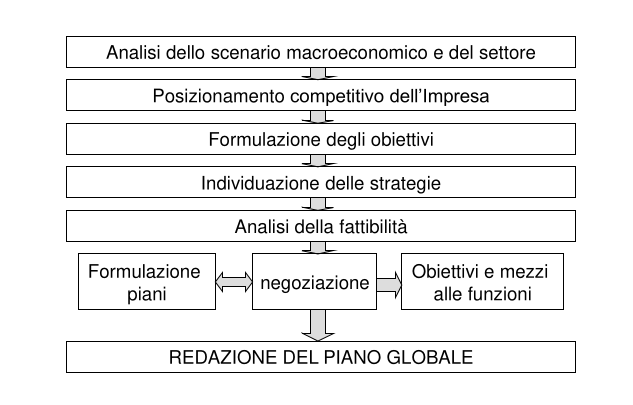
\includegraphics[width=0.5\linewidth]{1/img/Screenshot from 2022-07-04 17-21-38.png}
\end{figure}

\begin{figure}[H]
    \centering
    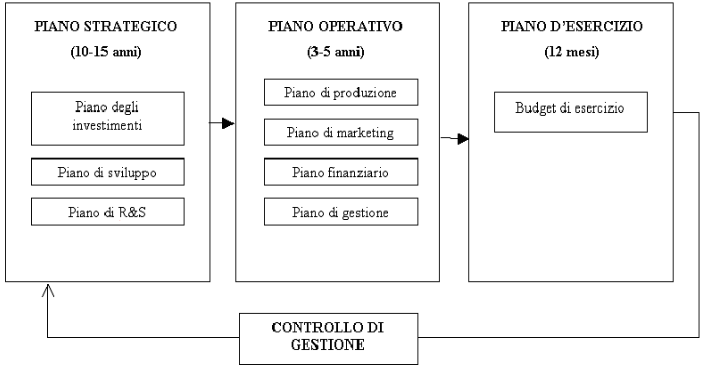
\includegraphics[width=0.5\linewidth]{1/img/Screenshot from 2022-07-04 17-22-15.png}
\end{figure}


\subsection{Gestione delle risorse umane}
Composta da gestione del personale e dall'organizzazione del personale.

L'organizzazione include la definizione di ruoli per il personale e l'assetto organizzativo in generale.


L'aspetto gestionale:
\begin{itemize}
    \item riperimento del personale
    \item selezione
    \item addestramento
    \item altre menate
\end{itemize}


    

\section{Il bilancio di esercizio}

\subsection{Concetto di azienda(riepilogo)}

\subsubsection{In termini soggettivi}
Istituto economico dotato di autonomia e proiettato nel tempo, in cui si coordinano una molteplicità
di risorse per il raggiungimento dei fini stabiliti dal soggetto istituzionale.

\subsubsection{In termini oggettivi}
Insieme delle attività svolte dall'istituto nell'ambiente economico(azione econimica).

Sistema di azioni che si traducono in scambi con terzi finalizzati al raggiungimento di un fine economico.


\subsubsection{Caratteristiche dei beni e servizi oggettivi di scambio}

Utilità(soddisfacimento dei bisogni).

Scarsità(determina il valore economico di transazione e rilevazione)


\subsection{Rilevazione: principali funzioni}

Quantificare, misurare, rappresentare e interpretare i fatti aziendali.

\subsection{Metodi per la rilevazione}
\textbf{Contabili}: si servono del conto quale strumento principale delle rilevazioni.

\textbf{Non contabili}: altri strumenti.

\subsection{Il sistema contabile e le informazioni}
Le informazioni a cui il sistema contabile si può riferire possono riguradare:
\begin{itemize}
    \item situazioni di economicità globale(prende un grosso periodo in analisi)
    \item situazioni parziali(analisi parziale dell'attività)
    \item situazioni attinenti al rapporto tra l'azienda e le principali categorie di interlocutori esterni
\end{itemize}

\subsection{Contabilità}
Raccolta. misurazione, analisi, interpretazione, sintesi e comunicazione di informazioni
economiche.

\subsection{Funzioni della contabilità generale}
Processo organico e sistematico di rilevazione di fatti di gestione,
scambi con terzi(fornitori e o clienti) e utlizza lo strumento della contabilità
e il metodo della partita doppia per:
\begin{itemize}
    \item determinazione periodica del risultato e del capitale di funzionamento
    \item controllo delle posizioni finaziarie azindali
\end{itemize}

\subsection{Le operazioni aziendali}
Sono operazioni di gestione che vengono fatte di continuo e in modo simultaneo:


\begin{itemize}
    \item sono unità elementari dell'attività operatia
    \item diversa complessità
    \item possono essere interpretate all'interno del sistema e non solo in modo individuale
\end{itemize}

\subsection{Processo di produzione economica}
gestione finalizzata a:
\begin{itemize}
    \item condizione di gestione(organizzazione)
    \item fattori produttivi: generici e specifici(investimenti in macchinari, impianti, ecc)
\end{itemize}


Il capitale messo a disposizione dall'imprenditore o dai soci è il capitale di rischio.

Il capitale di credito sono i prestiti che terzi(si spera banche) fanno all'azienda(non mafia ecco KEKW).

Per il capitale di rischio non c'è un obbligo di restituzione, viene conferito o come messi monetari
o direttamente aggiungendo fattori produttivi e può essere conferito in momenti differenti.

Per la remunerazione si deve vedere come va l'azienda.

Il capitale di terzi(prestiti) deve essere rimborsato nella maniera stabilità insieme al terzo in questione.


\subsection{Il circuito della produzione}
I mezzi moentari vengono investiti in fattori produttivi, la fase di produziione si divide in aquisizione materiale,
processamento e vendita.

\textbf{La differenza fra ricavi e costi è il reddito}


I prestiti non rappresentano variazione della ricchezza aziendale, si segna soltanto 
la differenza fra denaro ricevuto e quello restituito(l'interesse) che è alla fine dei 
conti l'unico esborso dell'azienda.



\begin{figure}[H]
    \centering
    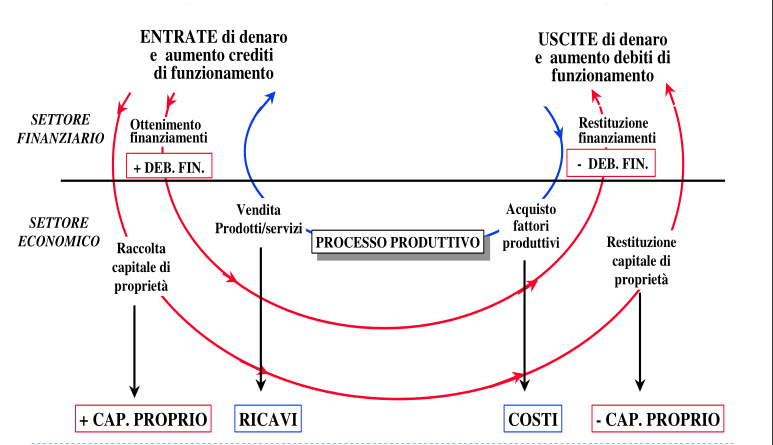
\includegraphics[width=0.7\linewidth]{2/img/Screenshot from 2022-07-05 15-52-30.png}
\end{figure}

\subsection{Classificazione variazioni di valore}
\subsubsection{Variazione finanziaria negativa}
\begin{itemize}
    \item diminuzione di denaro
    \item aumento debito funzionamento
    \item aumento debito finanziamento
    \item diminuzione credito funzionamento
    \item diminuzione credito finanziamento
\end{itemize}

\subsubsection{Variazione finanziaria positiva}
\begin{itemize}
    \item aumento di denaro
    \item aumento di crediti di funzionamento
    \item aumento di crediti fi finanziamento
    \item diminuzione debiti di funzionamento 
    \item diminuzione di debiti di finanziamento
\end{itemize}

\subsubsection{Variazione economica positiva}
\begin{itemize}
    \item ricavi
    \item rettifiche (diminuzione) dei costi
    \item aumento di capitale proprio
\end{itemize}

\subsubsection{Variazione economica negativa}
\begin{itemize}
    \item costi
    \item rettifiche(diminuzione) dei ricavi
    \item riduzione capitale prorpio
\end{itemize}

In sintesi:
\begin{itemize}
    \item Aspetto finanziario
        \begin{itemize}
            \item denaro
            \item credito e debito funzionamento
            \item credito e debito finanziamento
        \end{itemize}
    \item Aspetto economico
        \begin{itemize}
            \item costi
            \item ricavi
            \item capitale proprio
        \end{itemize}
\end{itemize}

\subsection{Aspetto finanziario ed economico dei fattori produttivi}
Divisione fra fattori produttivi che vengono usati una volta sola(fecondità semplice)
e altri fattori che vengono usati ripetutamente e perdono solo una porzione di valore al momento 
dell'utilizzo(fecondità ripetuta).

\subsubsection{Principio di correlazione}
Un fattore produttivo deve essere correlato alla realizzazione del prodotto che ha 
contribuito a creare.



\begin{figure}[H]
    \centering
    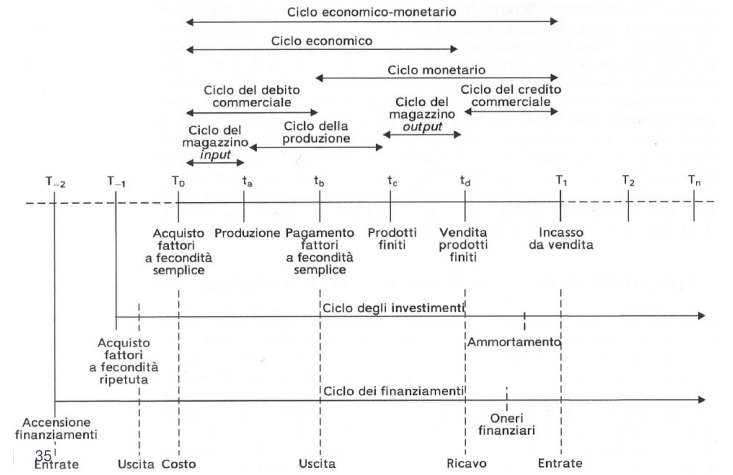
\includegraphics[width=0.7\linewidth]{2/img/Screenshot from 2022-07-05 16-11-59.png}
\end{figure}
\section{Bilancio di esercizio}
\subsection{Contabilità generale( Co. Ge)}

Insieme dei procedimenti informativi che utilizza lo
strumento contabile e il metodo della partita doppia

Ha lo scopo di rilevare i flussi finanziari e dei correlativi flussi economici.

\subsection{Il metodo della partita doppia}

\begin{itemize}
    \item istituire: fissare l'oggetto e la denominazione di un conto
    \item aprire o accendere: effettuare la prima registrazione
    \item chiudere: tirare la somma algebrica e scrivere nella sezione con totale minore, il valore per arrivare in pari fra le cose postive e quelle negative
    \item addebitare: iscrivere una variazione di conto in dare
    \item accreditare: iscrivere una variazione di conto in avere
    \item stornare: eliminare da un conto una quantità e trasferirla in un'altro conto
    \item riepilogare: trasferire il contenuto di più conti in uno di sintesi
    \item funzionmento antitetico dei conti(conti in sezioni diverse hanno segno opposto)
    \item duplicità dell'aspetto di osservazione
        \begin{itemize}
            \item ogni fatto dever essere osservato secondo un dulice aspetto(origine e derivato)
            \item di conseguenza si avranno conti accesi all'aspetto originario e conti accesi all'aspetto derivato
        \end{itemize}
    \item funzionamento antitetico delle classi di conti
\end{itemize}


Da queste regole deriva che:
\begin{itemize}
    \item la somma degli importi in dare di tutti i conti è uguale alla somma in avere di tutti i conti
    \item la somma dei saldi in dare di tutti i conti è uguale alla somma dei saldi in avere di tutti i conti
    \item la somma algebrica dei saldi in una parte qualsiasi dei conti del mastro è uguale e di segno opposto alla somma algebrica dei saldi della rimannente parte dei conti
\end{itemize}

\subsection{Metodo della partita doppia: rilevazione dei fatti di gestione}
\begin{itemize}
    \item valori finanziari
        \begin{itemize}
            \item denaro e valori assimilati
            \item crediti e debiti di funzionamento
            \item crediti e debiti di finanziamento
        \end{itemize}
    \item valori economici
        \begin{itemize}
            \item reddito(enttrate - uscite)
            \item capitale
        \end{itemize}
\end{itemize}

I valori finanziari in prevalenza si riferiscono all'aspetto
originario mentre i valori economici si riferiscono
all'aspetto derivato di osservazione.

Le classi di conto sono due: conti finanziar(aspetto originarioi) e conti economici(aspetto derivato).


\subsubsection{Conti finanziari}
Accolgono in dare le variazioni positive e in avere le variazioni negative.

\subsubsection{Conti economici}
Accolgono in dare le variazioni negative e in avere le variazioni positive.

\subsection{Il modello del bilancio}
Il bilancio di esercizio ha lo scopo di determianre e di rappresentare le condizioni di equilibrio
economico, finaziario e patrimoniale dell'azienda.

Offre infromazioni sul risultato economico di un singolo periodo(31/12).


Il risultato economico di periodo si forma mediante le operazioni di gestione dell'attività.

Serve a misurare il variare della ricchezza di un periodo.


Il risultato economico globale è il risultato conseguito durante tutto il periodo di vita dell'azienda(sommo tutti i risultati di periodo).

\begin{figure}[H]
    \centering
    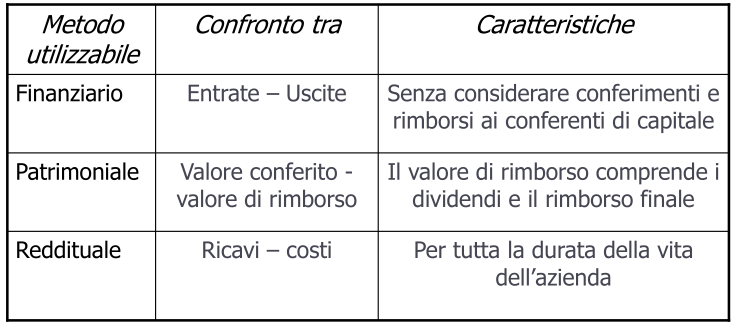
\includegraphics[width=0.7\linewidth]{2/img/Screenshot from 2022-07-06 15-27-34.png}
\end{figure}

\subsection{Costo di acquisizione e costo di utilizzazione}

Il costo di acquisizione è il costo speso per un certo fattore produttivo(ferro, macchinario, ecc).


Il costo di utilizzazione è il valore dei fattori produttivi che vengono usati nella realizzazione
di un prodotto o di un servizio che hanno generato un ricavo.


La differenza tra costo di acquisizione(dinamica monetaria) e costo di utilizzo(dinamica economica)
 di un fattore produttivo a fecondità ripetuta rappresenta il valore residuo del fattore produttivo, il che implica che ci siano
 ancora operazioni possibili con un certo asset.

 \subsection{Ammortamento}
 La quota di ammortamento rappresenta il valore che può essere fatto partecipare in componente negativa 
 al risultato economico di periodo.

 In questo modo i fattori produttivi vengono suddivisi sul periodo nel quale vengono utilizati.

 \subsection{Il principio di competenza}
 Sono di competenza di un periodo i costi ed i ricavi dei processi compiuti:
 \begin{itemize}
    \item conclusi con il conseguimento dei ricavi
    \item con la condizione che nello stesso periodo si sia effettuata anche la prestazione
 \end{itemize}

 \subsection{Principio di prudenza}
 Il risultato economico di periodo è un valore astratto e non implica le disponibilità
 di cassa dell'azienda.

 Per trasferire la ricchezza prodotta ai conferenti di capitale di rischio senza che si
 svuotino le casse della gestione si devono considerare le perdite anche se solo temute e
 non considerare i ricavi se solo sperati.

 \subsection{Capitale di funzionamento}

 Al termine di un periodo rimangono fattori produttivi:
 \begin{itemize}
    \item generici(denaro, risorse finanziarie)
    \item specifici(prodotti da usare, cicli produttivi da terminare e prodotti da vendere)
 \end{itemize}

 \subsection{Il modello del bilancio}
 il modello economico finanziario consente di misurare e rappresentare l'economicità(equilibrio economico, patrimoniale e finaziario),
 rispettando delle condizioni:
 \begin{itemize}
    \item efficacia(raggiungere gli obiettivi)
    \item efficienza(minor risorse usate per l'obiettivo)
 \end{itemize}

 Queste cose vengono analizzate dal modello del bilancio.


 \begin{itemize}
    \item Oggetto dedl bilancio
        \begin{itemize}
            \item insieme dei valori economici e finanziari che derivano dalla gestione e rappresentano variazioni delle risorse
        \end{itemize}
    \item finalità del bilancio
        \begin{itemize}
            \item rappresentazione chiara, veritiera e corretta della situazione patrimoniale e finanziaria della società e del risultato economico.
        \end{itemize}
    \item prospetti fondamentali
        \begin{itemize}
            \item stato patrimoniale
            \item conto economico
            \item (rendiconto finaziario)
        \end{itemize}
 \end{itemize}

 \subsection{Stato patrimoniale}
 Descrive la situazione patrimoniale in certo istante.

 \begin{itemize}
    \item valore monetario misurabile = \textbf{attività}
    \item diritti vantati da terzi = \textbf{passività}
    \item diritti vantati dai soci = \textbf{patrimonio netto}
 \end{itemize}

 Il valore attività è forato dalla somma del patrimonio netto e delle passività.

 \subsubsection{Struttura sintetica}
 \begin{figure}[H]
    \centering
    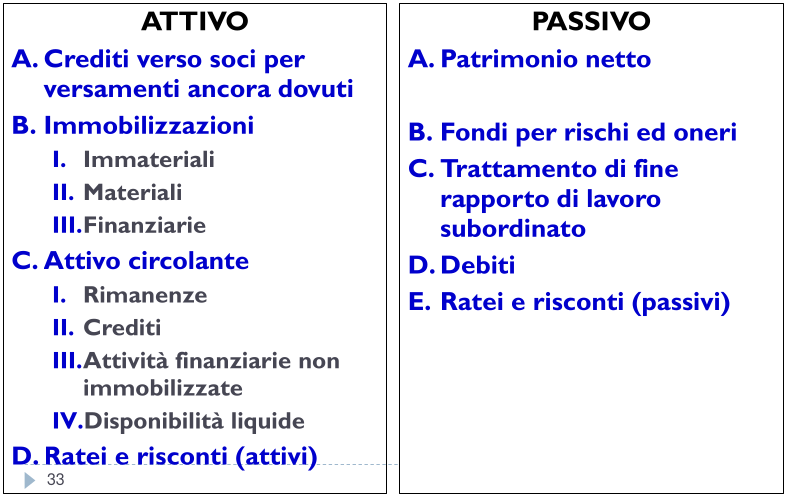
\includegraphics[width=0.7\linewidth]{2/img/Screenshot from 2022-07-06 16-07-29.png}
\end{figure}

\subsection{Conto economico}

Sintesi dei flussi di natira economica(ricavi e costi) che interessano l'impresa in un certo intervallo temporale.

Evidenzia la progressiva formazione del risultato economico di periodo.

\subsubsection{Struttura sintetica}
\begin{figure}[H]
    \centering
    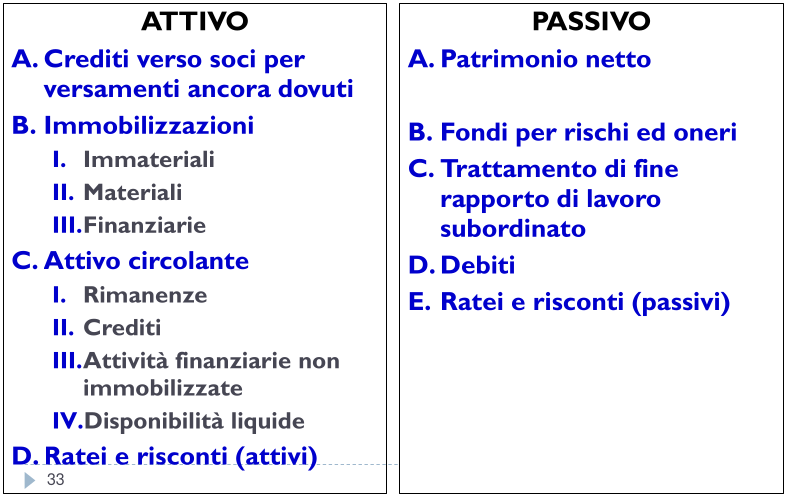
\includegraphics[width=0.7\linewidth]{2/img/Screenshot from 2022-07-06 16-07-29.png}
\end{figure}

\section{I principi contabili di base}
\subsection{Omogeneità}
Le registrazioni contabili si riferiscono solo a eventi che producono qualcosa quantificabile in termini monetari.

I termini inseriti sono in termini di potere d'acquisto della moneta in quel momento storico
(c'è da fare un'interpretazioni con il passare degli anni).


\subsection{Entità}

La contabilità si riferisce ad un'entità e non alle persone ad essa collegate.


\subsection{La prospettiva di continuità di funzionamento}
Si deve assumere che un'azienda continui all'infinito.

In caso si voglia chiudere si fa un bilancio di liquidazione e non un bilancio di esercizio.s


\subsection{Costo}
Un'attività è rilevata in contabilità al suo prezzo d'acquisto cioè al \textbf{costo storico}.

Le attività poi si possono dividere in monetarie e non, le monetarie hanno un'informazione
oggettiva sul valore (\textbf{fair value}), invece, le attività che non hanno un valore oggettivo(terreni, fabbricati, macchinari) per queste si tiene in considerazione il \textbf{costo storico(prezzo di acquisto iniziale)}.

Ovviamente il costo storico nel corso degli anni viene modificato a scendere.



\subsection{Duplice aspetto}

L'attività è la somma di passività e capitale netto
\subsection{Periodo della misurazione}
Si cerca di avere una periodicità nelle misurazioni in modo da capire l'andamento dell'azienda
e aggiustare il tiro.

Il periodo amministrativo va dal 1 Gennaio al 31 Dicembre.


\subsection{Prudenza}
Si devono trattare i dati con ragionevole scetticismo di modo da aumentare la credibilità dei risultati.


\textbf{prudenza}: attitudine a sottostimare il reddito e le attività
qualora sussita incertezza.

Applicando la prudenza si ha che:
\begin{itemize}
    \item I ricavi(aumento utili) si riconoscono solo quando sono ragionevolmente certi
    \item riconoscere i costi(diminuzione di utili) non appena sono ragionevolmente possibili
\end{itemize}

I ricavi sono normalmente riconosciuti all consegna del prodotto al cliente.



\subsection{Realizzazione dei ricavi}

Quanto ricavo devo riconoscere??

Quello che il cliente con ragionevole certezza pagherà.


\subsection{Competenza}

Un costo di competenza di un certo periodo è un costo da associare a
quel periodo amministrativo, rappresenta risorse consumate nel
periodo per la produzione dei ricavi del periodo.

Sono necessarie operazioni di rettifica.


\subsection{Continuità dei criteri di valutazione}

Una volta adottato un metodo di valutazione devo rimanere con quello, cosi da evitare di fare conversioni tra metdoti e introdurre errori.

In questo modo è anche possibile confrontare bilanci di periodi diversi con facilità.


\subsection{Significità e rilevanza}

\begin{itemize}
    \item Trascurare le transazioni irrilevanti
    \item individuare l transazioni rilevanti
\end{itemize}

Sono rilevanti le transazioni che, se fossero contabilizzate, indurrebbero a valutare diversamente il bilancio.


\section{Il bilancio di esercizio}
\begin{figure}[H]
    \centering
    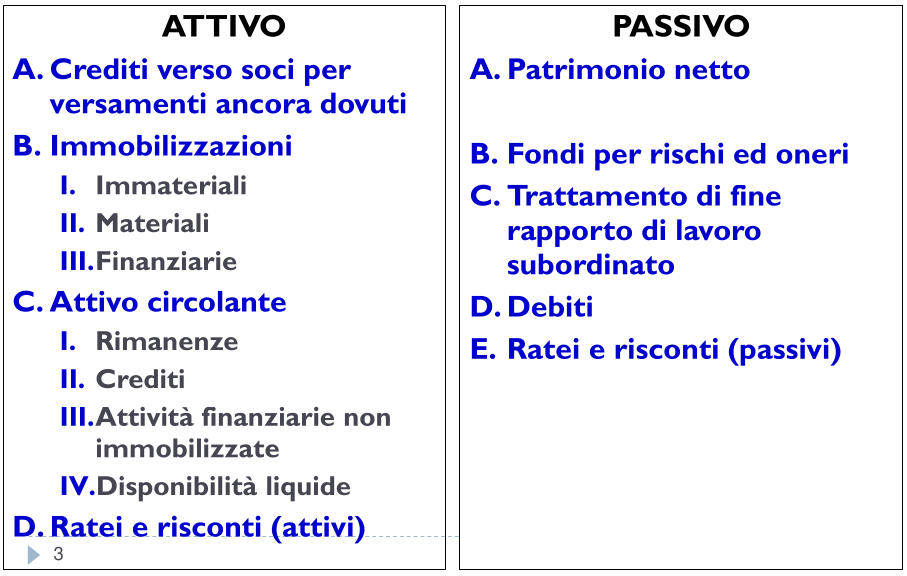
\includegraphics[width=0.7\linewidth]{2/img/Screenshot from 2022-07-06 22-20-49.png}
\end{figure}
\subsection{Stato patrimoniale: Attività}


\subsubsection{Crediti verso soci per versamenti ancora dovuti}

è 0 se il capitale sociale è stato versato dai soci.

\subsubsection{Immobilizazzione}
Immobilizzazioni immateriali:
\begin{itemize}
    \item costi di impianto e di ampliamento
    \item costi di sviluppo
    \item diritto di brevetto
    \item concessioni, licenze, marchi e diritti simili
    \item avviamento
    \item immobilizzazi in corso e acconti
    \item altre
\end{itemize}

Immobilizzazioni materiali:
\begin{itemize}
    \item terreni e fabbricati
    \item impianti e macchinari
    \item attrezzature
    \item altri begin
    \item Immobilizazzione in  corso e acconti
\end{itemize}


Immobilizzazioni finanziarie:
\begin{itemize}
    \item partecipazioni in imprese
    \item Creditialtri titoli
    \item strumenti finanziari derivati attivi
\end{itemize}

\subsubsection{Attivo circolare}
rimanenze:
\begin{itemize}
    \item materie prime ecc
    \item prodotti in corso di lavorazione
    \item lavori in corso
    \item prodotti finiti e merci
    \item acconti
\end{itemize}

crediti:
\begin{itemize}
    \item verso cliente
    \item verso imprese controllate
    \item verso imprese collegate
    \item verso imprese controllanti
    \item crediti tributari
    \item imposte anticipate
\end{itemize}

Attività finanziarie che non costituiscono immobilizzazioni:
\begin{itemize}
    \item patecipazione non strategica in aziende
    \item altre partecipazioni
    \item strumenti derivati attivi
\end{itemize}

Disponibilità liquide:
\begin{itemize}
    \item depositi bancari e postali
    \item assegni
    \item denaro e valori in cassa
\end{itemize}


\subsubsection{Ratei e riscontri(attivi)}
I ratei attivi rilevano quote di ricavi di competenza dell'esericzio in corso
esigibili nell'esercizio successivo.

I riscontri attivi rettificano quote di costo già rilevate ma di competenza di esercizi passati.


\subsection{Stato patrimoniale: Passività}
\subsubsection{Patrimonio netto}
Insieme delle fonti di capitale proprio(di rischio)
\begin{itemize}
    \item capitale
    \item risetva da sovrapprezzo delle azioni
    \item riserva di rivalutazione
    \item riserva legale
    \item utili(perdite) portati a nuovo
    \item itili(perdita) dell'esercizio
    \item riserva negativa per azioni prorpie in portafoglio 
\end{itemize}

\subsubsection{Fonti per rischi ed oneri}

Soldi da parte per:
\begin{itemize}
    \item quiescenze e robe simili
    \item imposte
    \item strumenti finanziari derivati Passività
    \item altro
\end{itemize}

\subsubsection{TFR dei lavoratori}
accantonamento dei soldi maturati dal dipendente dati via al momento del licenziamento.

\subsubsection{Debiti}
\begin{itemize}
    \item obbligazioni
    \item debiti verso qualcuno
    \item acconti
\end{itemize}

\subsubsection{Ratei e riscontri(passivi)}
I ratei passivi rilevano i quote di costi di competenza dell'esercizio esigibili nell'esercizio successivo.

I risconti passivi rettificano quote di ricavo già rilevate ma
di competenza dell'esercizio successivo.


\subsection{Il conto economico}
\begin{figure}[H]
    \centering
    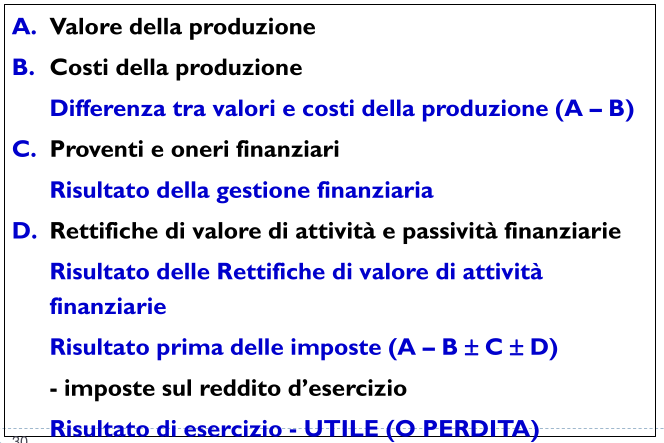
\includegraphics[width=0.7\linewidth]{2/img/Screenshot from 2022-07-07 16-11-55.png}
\end{figure}

\subsubsection{Valore della produzione}
valore di tutti i beni prodotti dall'impresa nell'esercizio
\begin{itemize}
    \item ricavi dalle vendite e delle prestazioni
    \item variazioni delle rimanenze di prodotti in lavorazione
    \item variazioni dei lavori in corso su ordinazione
    \item incremento di immobilizzazione per lavori interni
    \item altri ricavi e proventi
\end{itemize}

\subsubsection{Costi della produzione}
insieme dei costi sostenuti dall'impresa, derivanti sia da attività di
vera e propria trasformazione, sia da attività di supporto.


\begin{itemize}
    \item materie prime
    \item servizi
    \item personale(salari ecc)
    \item ammortamentie svalutazioni
    \item variazione delle rimanenze di magazzino
    \item accantonamento rischi
    \item oneri diversi di gestione
\end{itemize}

\subsubsection{Differenza tra valori e costi della produzione}
MON = margine operativo netto, è il risultato dell'attività operativa dell'impresa.


VAL = valore aggiunto lordo, misura quanto la gestione operativa dell'impresa ha aumentato il valore degli acquisti.

\subsubsection{Proventi e oneri finanziari}
\begin{itemize}
    \item proventi da partecipazioni
    \item interessi e altri oneri
    \item utili e perdite su scambi
\end{itemize}

\subsubsection{Rettifiche di valore di attività e passività finanziarie}
\begin{itemize}
    \item rivalutazione di partecipazioni
    \item svalutazione di partecipazioni
\end{itemize}


\subsection{Conto economico}
Il risultato prima delle imposte è:
\textbf{Valore della produzione - Costi della produzione $\pm$ proventi e oneri finanziari $\pm$ Retifiche di valore di attività e passività finanzirie
}

Successivamente \textbf{si sottraggono le imposte sul reddito d'esercizio} e \textbf{si ottengono
risultato di esercizio(UTILE o PERDITA)} 


\section{Il bilancio di esercizio}
\subsection{Il modello del bilancio: Archetipo economico-finanziario}

\begin{figure}[H]
    \centering
    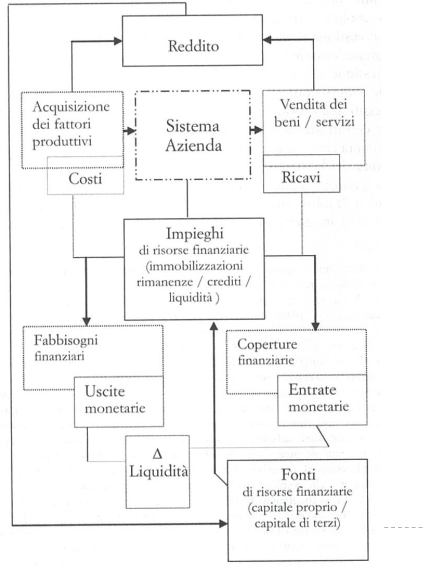
\includegraphics[width=0.4\linewidth]{2/img/Screenshot from 2022-07-09 16-49-15.png}
\end{figure}

\subsection{Il modello del bilancio: I prospetti numerici}


\begin{figure}[H]
    \centering
    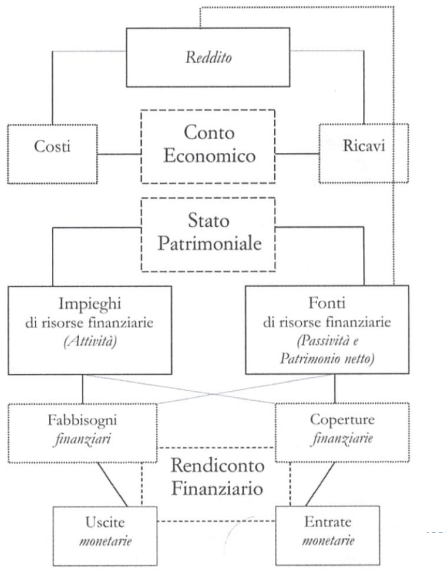
\includegraphics[width=0.4\linewidth]{2/img/Screenshot from 2022-07-09 16-50-17.png}
\end{figure}

\subsection{Classificazione delle voci in base alla determinazione dei valori}
\begin{figure}[H]
    \centering
    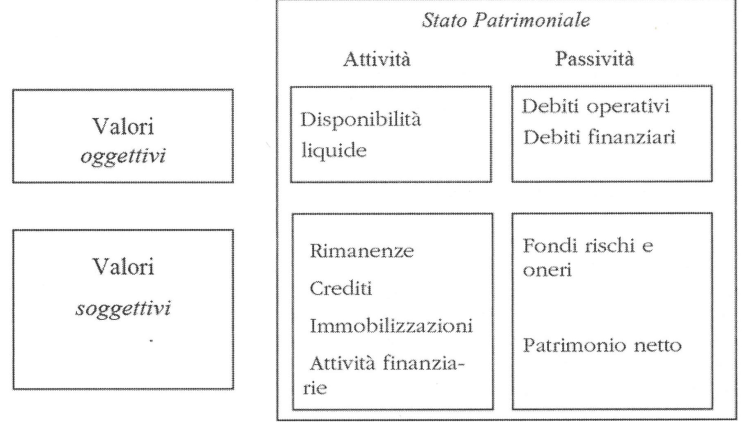
\includegraphics[width=0.4\linewidth]{2/img/Screenshot from 2022-07-09 18-21-32.png}
\end{figure}
\begin{figure}[H]
    \centering
    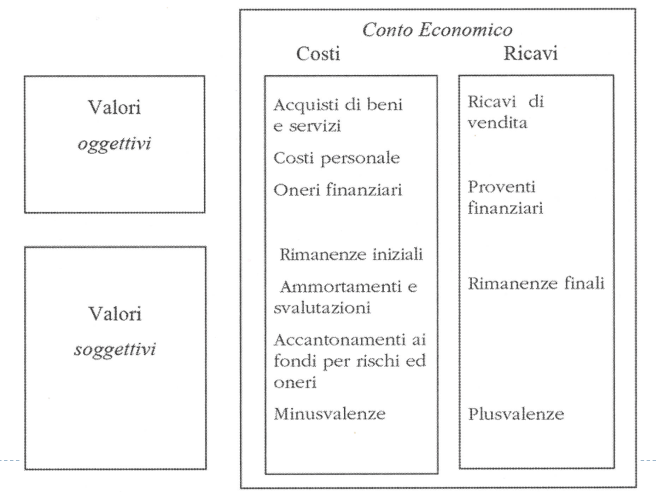
\includegraphics[width=0.4\linewidth]{2/img/Screenshot from 2022-07-09 18-22-41.png}
\end{figure}

\subsection{Analisi del bilancio}
Analizzare i dati contabili ed extra-contabili per valutare e giudicare la gestione aziendale.

Si confrontano i dati di più bilanci per avere una cmparazione temporale(stessa impresa) o comparazione spaziale(differenti aziende).

L'analisi del bilancio è volta a determinare lo stato di salute dell'azienda sulla base
si tre fattori che devono mantersi in equilibrio fra di loro:
\begin{itemize}
    \item economico: produrre reddito per periodo ampio e remunerare i fattori produttivi
    \item patrimoniale: equilibrio tra attività e passività + patrimonio netto
    \item finanziario: rispondere in modo tempestivo agli impegni assunti
\end{itemize}

\subsection{Analisi di bilancio: prospettive}
\begin{figure}[H]
    \centering
    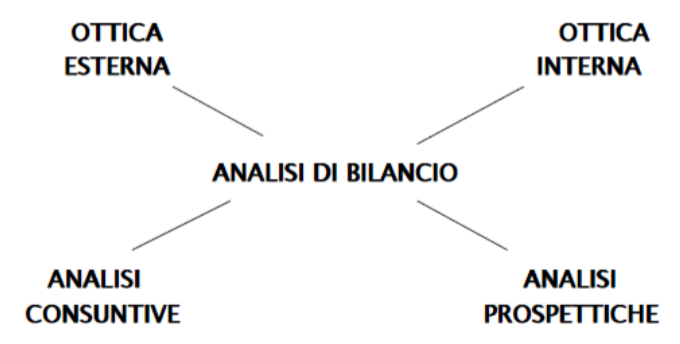
\includegraphics[width=0.5\linewidth]{2/img/Screenshot from 2022-07-10 10-42-56.png}
\end{figure}

\subsubsection{Articolazione}
\begin{figure}[H]
    \centering
    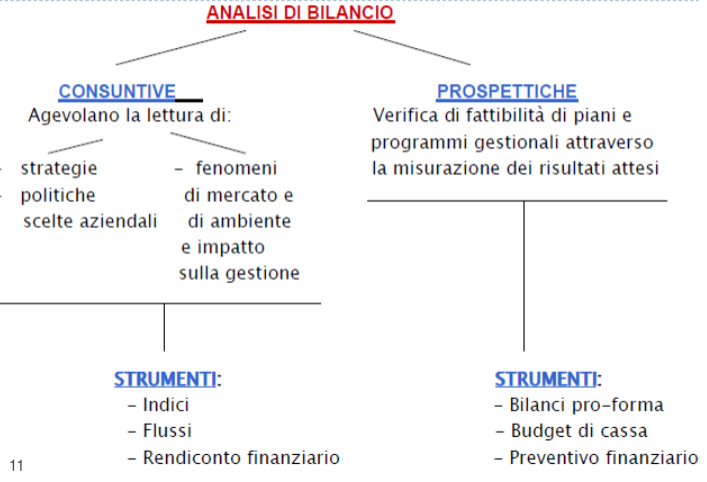
\includegraphics[width=0.5\linewidth]{2/img/Screenshot from 2022-07-10 10-47-54.png}
\end{figure}

\subsubsection{Analisi di bilancio: ottica}
Analisi interne: 
\begin{itemize}
    \item basate sulla documentazione aziendale
    \item completo e tempestivo
    \item riservatezza dei dati permette un bilancio migliore
\end{itemize}


Analisi esterne: 
\begin{itemize}
    \item basato sul bilnacio pubblico
    \item esigenze di riservatezza sull'informazioni(qualità inferiore)
\end{itemize}

\subsubsection{Fasi dell'analisi di bilancio}
\begin{enumerate}
    \item Ricerca ei dati contabili ed extracontabili e loro interpretazioni
    \item riclassificazione dello stato patrimoniale e del conto economico
    \item analisi per indici
    \item analisi per flussi
    \item valutazione dei risultati
\end{enumerate}

Raggruppando le voci di bilancio in gruppi omogenei si facilità il compito di confronto con valori precedenti dei dati e si migliora la lettrua critica.


\subsection{Riclassificazione del conto economico}
Dati aggregati in:
\begin{itemize}
    \item gestione caratteristica(o operativa): costi e ricavi dell'attività di acquisto, trasformazione e vendita
    \item gestione extra-caratteristica(o extra-operativa): 
        \begin{itemize}
            \item gestione accessoria(o straordinaria): attività continuative con con sono l'obiettivo dell'azienda
            \item gestione finanziaria: risultati di operazioni di reperimento di capitale e dell'investimento di risorse liquide
            \item gestione fiscale: elementi di natura fiscale
        \end{itemize}
\end{itemize}

Il principio comune è quello di separare le caratteristiche operative da quelle extra-operative.


Avendo il \textbf{ricavo netto di vendita}, si sottrae il \textbf{costo dei prodotti venduti} e si ottiene 
il \textbf{risultato lordo}.

Poi si sottraggono dal \textbf{risultato lordo} tutte le spese e si ottiene il \textbf{risultato operativo}.

\subsection{Conto Economico a ricavi e costo del
venduto: gestione extra-caratteristica}

\begin{figure}[H]
    \centering
    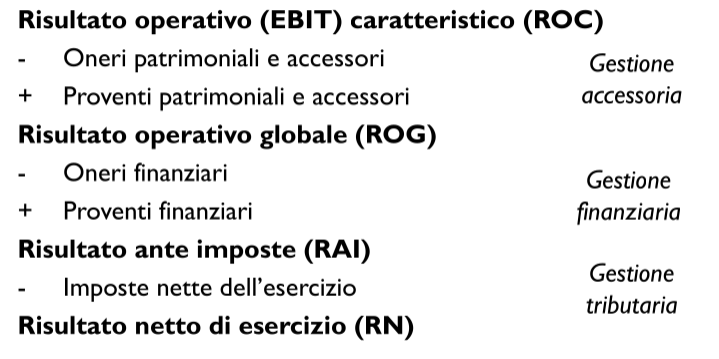
\includegraphics[width=0.5\linewidth]{2/img/Screenshot from 2022-07-10 11-21-34.png}
\end{figure}

\subsection{Conto economico a valore aggiunto}
Ordina i costi per natra economica, la classificaione è in linea con quello civilistica, eichiede meno informazioni rispetto
al conto economico a ricavi e costi del venduto ed è preferito dagli analisti esterni.


\begin{figure}[H]
    \centering
    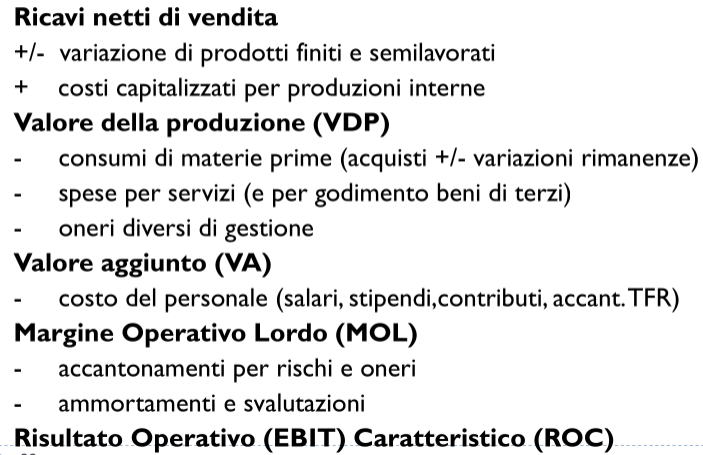
\includegraphics[width=0.5\linewidth]{2/img/Screenshot from 2022-07-10 11-33-38.png}
\end{figure}


\section{Da rifare per bene}
\section{Il bilancio di esercizio}
\subsection{Circolare capitale netto}
Rappresenta la quota di capitale di esercizio finanziaria con risorse a disposizione dell'azienda in via stabile e permanente.

Rappresentata da differenza tra attività a breve e passività a breve.

\subsection{Margine di tesoreria}
(Attività correnti - magazzino netto) - Passività correnti

Capacità dell'impresa di fare fronte a cose con solo le liquidità immediate.

\subsection{Margine di struttura}
Capitale netto - immobilizzazione nette

\subsection{Indici di bilancio}
La liquidità di un'azienda è data dalla sua capacità di onorare le obbligazioni che scadono nel breve(solvibilità a breve).

\begin{equation*}
    \text{Indice di liquidità corrente o disponibilità} = \frac{\text{Attivo corrente}}{\text{Passivo corrente}}
\end{equation*}

\begin{itemize}
    \item $\geq 1,5$ equilibrio
    \item $> 1, < 1,5$ attenzione
    \item $< 1$ squilibrio
\end{itemize}

\subsection{Indice Indice di liquidità immediata}
\begin{equation*}
    \text{Indice di liquidità immediata} = \frac{\text{Attivo corrente} - \text{Rimanenze}}{\text{Passivo corrente}}
\end{equation*}

\begin{itemize}
    \item tra 0,5 e 1 situazione di equilibrio
    \item tra 0,33 e 0,5 attenzione
    \item se sotto 0,33 situazione di squilbrio
\end{itemize}

\subsection{Indici di solidità patrimoniale}
Permettono di capire la solvibilità a medio lungo termine.

\subsubsection{Tasso di indebitamento Leverage(D/E)}
\begin{equation*}
    \text{D/E} = \frac{\text{Mezzi di terzi}}{\text{Patrimonio netto}} \leq 1
\end{equation*}

\subsubsection{Indice di autocopertura delle immobilizzazioni}
Il patrimonio netto copre le immobilizzazioni
\begin{equation*}
    \text{Indice di autocopertura delle immobilizzazioni} = \frac{\text{Patrimonio netto}}{\text{Immobilizzazione}}
\end{equation*}

\begin{itemize}
    \item $\geq 0,7$ equilibrio
    \item $< 0,7$ attenzione
    \item $< 0,5$ squilibrio
\end{itemize}

\subsubsection{Indice di copertura delle immobilizzazioni}
Gli investimenti sono coperti delle fonti finanziarie a lungo termine.

\begin{equation*}
    \text{Indice di copertura delle immobilizzazioni} = 
    \frac{
        \text{Debiti a m/l termine} + \text{Patrimonio netto}
    }{
        \text{Immobilizzazioni}
    }
\end{equation*}

\begin{itemize}
    \item $\geq 1,5$ equilibrio
    \item $< 1,5$ attenzione
    \item $< 1$ squilibrio
\end{itemize}

\subsubsection{Indice di indipendenza finanziaria(IIF)}
\begin{equation*}
    \text{IIF} = \frac{\text{Patrimonio netto}}{\text{Attivo netto}}
\end{equation*}

\begin{itemize}
    \item 1 ideale
    \item tra 0,5 e 0,75 equilibrio
    \item sotto 0,5 squilibrio
\end{itemize}

\subsection{Indici di redditività}
Capacità di produrre utile attraverso lo svolgimentodell'impresa.

\subsubsection{ROE(return of equity)}
\begin{equation*}
    \text{ROE \%} = \frac{\text{Reddito netto}}{\text{Patrimonio netto}}
\end{equation*}

\subsubsection{IDEO - Incidenza gestione extra-operativa}
\begin{equation*}
    \text{IGEO} = \frac{\text{Reddito netto}}{\text{Risultato operativo (EBIT) Aziendale}}
\end{equation*}

\subsubsection{ROA - return on net asset}
\begin{figure}[H]
    \centering
    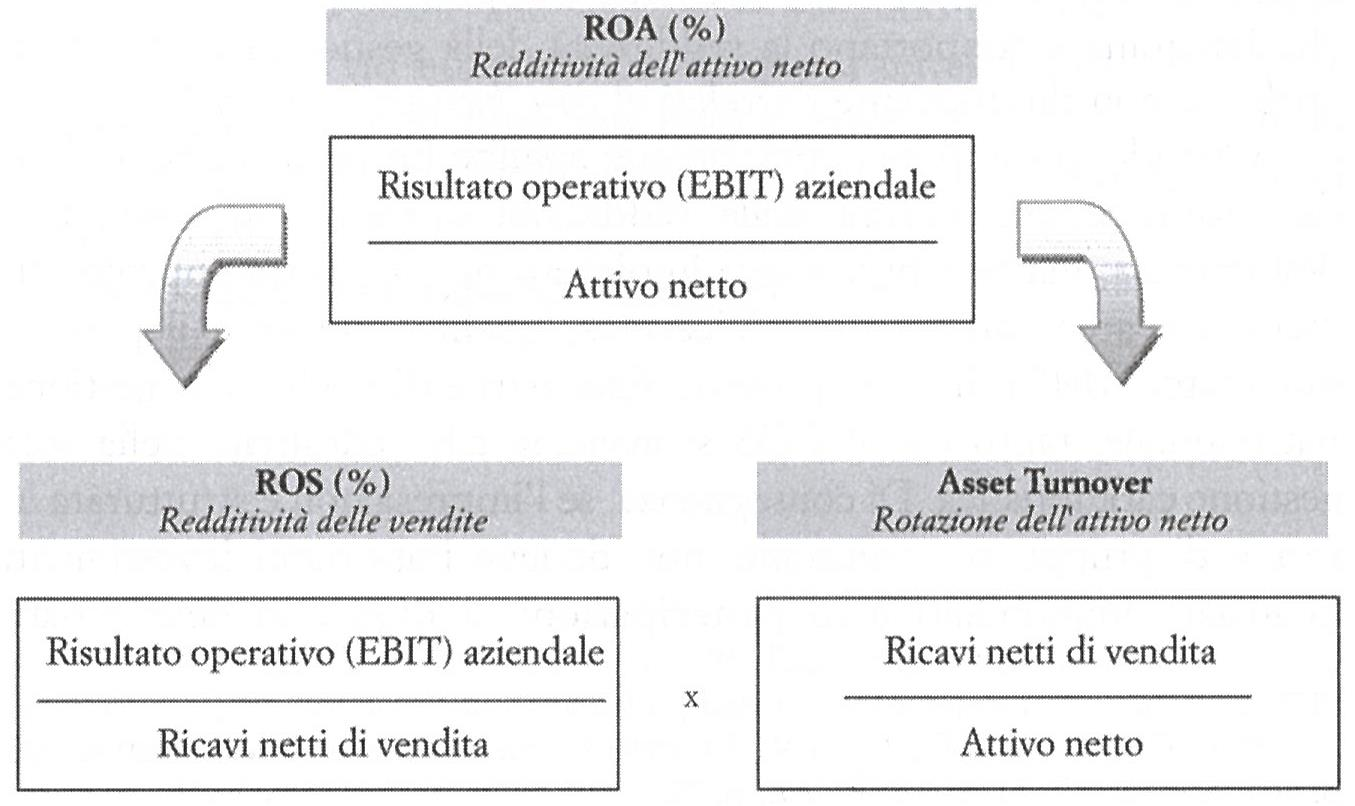
\includegraphics[width=0.7\linewidth]{2/img/ROA.png}
\end{figure}
\begin{equation*}
    \text{ROA \%} = \frac{\text{Risultato operativo (EBIT) aziendale}}{Attivo netto}
\end{equation*}

\subsubsection{Asset turnover}
Indica l'intensità con la quale l'azienda sfrutta i sui investimenti in attività operative.

\begin{equation*}
    \text{Asset Turnover} = \frac{\text{Ricavi netti}}{\text{Attivo netto}}
\end{equation*}

\subsubsection{ROS - Retunr on sales}
\begin{equation*}
    \text{ROS \%} = \frac{
        \text{
            Risultato operativo (EBIT) aziendale
        }
    }{
        \text{
            Ricavi netti
        }
    }
\end{equation*}

\subsubsection{ROD - return on debit}

\begin{equation*}
    \text{ROD \%} = \frac{
        \text{
            Oneri finanziari
        }
    }{
        \text{
            Mezzi di terzi
        }
    }
\end{equation*}

\subsubsection{Tasso di incidenza della gestione fiscale (t)}
\begin{equation*}
    t = \frac{
        \text{
            imposte sul reddito
        }
    }{
        \text{
            risultato ante imposte
        }
    }
\end{equation*}

\begin{equation*}
    \text{
        reddito netto
    } = \text{
        risultato ante imposte 
    }
    (1 - t)
\end{equation*}

\subsubsection{Leva finanziaria}
\begin{equation*}
    \text{ROE} = \frac{
        \text{
            RN
        }
    }{
        \text{
            RAI
        }
    } \Big[\text{ROA} + \Big(\text{ROA} - \text{ROD}\Big) \frac{\text{MT}}{\text{PN}}\Big]
\end{equation*}

\begin{itemize}
    \item \textbf{RN/RAI}: risutlato netto fratto risultato ante imposte
    \item \textbf{ROA}: Indice return on asset
    \item \textbf{MT}: debiti di finanziamento ad interesse esplicito
    \item \textbf{PN}: patrimonio netto
    \item \textbf{MT/MN}: indice di indebitamento (\textbf{D/E})
    \item \textbf{ROD}: oneri finanziari fratto debiti
\end{itemize}

Altre versione per scrivere questa cacata è quello di sostituire $\frac{\text{RN}}{\text{RAI}}$ con 
$(1 - t)$, si ottiene:
\begin{equation*}
    \text{ROE} = 
    \Big[\text{ROA} + \Big(\text{ROA} - \text{ROD}\Big) \frac{\text{MT}}{\text{PN}}\Big] (1 - t)
\end{equation*}

\begin{itemize}
    \item \textbf{$t$}: tasso di incidenza della gestione fiscale
\end{itemize}

ROA è maggiore di ROA solo se ROA è maggiore di ROD, leffetto della leva risulta:
\begin{equation*}
    \text{ROA} - \text{ROD} > 0
\end{equation*}

Così si ottiene una leva positiva, ma se ROD è maggiore di ROA, si ottiene una leva negativa!!


\section{Fai gli esercizi del pdf 2.5.1}

\section{I costi}

\subsection{L'attività d direzione nelle imprese}

Dirigere significa prednere dicisioni per garantire l'efficacia e l'effcienza ai processi che formano la combinazione produttiva.

\subsection{Contabilità generale VS analitica}

\begin{figure}[H]
    \centering
    \includegraphics[width=0.7\linewidth]{3/img/contabilità generale vs analitica.png}
\end{figure}

\subsection{Il concetto di costo}

Valore monetario necessario epr lo svolgimento di un'operazione.


Si possono fare calcoli di costo finali che coprono un'intero processo produttivo oppure 
si calcola l'oogetto intermendio cioè ogni singola fase.

\subsection{Diverse connfigurazioni di costo}
\begin{itemize}
    \item costo primo
    \item costo di trasformzaione
    \item costo perno di produzione
    \item costo pieno aziendale
\end{itemize}

\subsection{Diverse classi di costo}
\begin{itemize}
    \item costi diretti e costi indiretti
    \item costi variabili e costi fissi
    \item costi comuni e costi congiunti
    \item costi di prodotto e costi di periodo
\end{itemize}

\subsection{Costi diretti e indiretti}
\subsubsection{Costi diretti}
Costi dei fattori produttivi utilizzati in via esclusiva per l'ottenimento di un prodotto.


\subsubsection{Costi indiretti}
Costi di fattori produttivi (generalemente strutturali) usati alternativamente o contemporaneamente
per la produzione di più prodotti.

\subsection{Costi variabilie e costi fissi}
\subsubsection{Costi variabili}
Costi che variano al variare dei volumi di produzione.

Se questa variazione non cresce in modo lineare ma ha una variabilità crescente o decrescente, 
prende il nnome di cvu(costo variabile unitario) crescente o decrescente.

\subsubsection{Costi fissi}
Costi che non cambinao in base al volume produttivo come l'affitto del capannone o robe di questo tipo.

\subsection{Intervallo di rilevanza}
È l'intervallo di attività o di volume all'interno del quale si suppone
valida una specifica relazione fra il livello di attività/volume e il costo.


\subsection{Periodo temporale di rilevanza}
I costi sotenibili dipendono dalla finestra temporale:
\begin{itemize}
    \item brevissimo periodo: quasi tutti i costi non sono modificabili
    \item breve/medio periodo: alcuni costi modificabili
    \item lungo periodo: quasi tutti i costi modificabili
\end{itemize}

\subsection{Stima della relazione costo-volume}
CT(costo totale) = CFT(Costo fisso totale) + cvu(costo variabile unitario) * X(numero di prodotti)

\subsection{Costi eliminabili e costi ineliminabili}
I costi eliminabili sono quesi costi che se un prodotto dovesse essere eliminato dalla produzione verrebbero meno.

I costi non eliminabili sono uesi costi che anche se un prodotto venisse eliminato non scomparirebbero.

\subsection{Le configurazioni di costo}
\subsubsection{Direct cost}
Il costo di prodotto dipende solo dai costi diretti.

\subsubsection{Full cost(o costo pieno)}
Il costo di prodotto è composto da costi diretti e da quote di costi indiretti attribuiti utilizzando 
delle basi di ripartizione.

\subsubsection{Calcolo costo unitario di prodotto: costi diretti}
Prezzo di aqusto del fattore produttivo * quantità del fattore produttivo consumata per unità di prodotto = costo diretto dell'unità di prodotto.

\subsubsection{Calcolo costo unitario di prodotto: costi indiretti}

Costo indiretto / base di ripartizione = coefficiente di attribuzione.


Coefficiente di attribuzione * quota della base di ripartizione consumata dall'unità di prodotto = quota di costo indiretto per unità di prodotto.

\subsection{Orientamento ai fattori produttivi}
Le singole voci di costo sono raggruppate per categorie di fattori produttivi come:
\begin{itemize}
    \item costo alvoro indiretto
    \item ammortamenti industriali
    \item ammortamenti non industriali
    \item costo lavoro non industriale
    \item affitto e costi di struttura
    \item ecc
\end{itemize}

\subsection{Orientamento funzionale}
stessa cosa d quella sopra ma si aggregano i costi in base a:
\begin{itemize}
    \item costi indiretti di produzione
    \item costi commerciali
    \item costi amministrativi
    \item costi generali
    \item ecc
\end{itemize}

\subsection{Gerarchia centri di costo}
\begin{itemize}
    \item centri di produzione: processi di trasformazione
    \item centri ausiliari: fornisce robe agli altri centri di costo
    \item centri di servizi: esternia all'area produttiva(area comemrciale, amministrativa, ecc)
    \item centri virtuali: costi residuali per far quadrare i conti
\end{itemize}

\subsubsection{Medoto diretto}
si ipotizza una relazione diretta di ciascun centro
di servizi con i centri di costo di produzione.

Il pregio di questo metodo è rappresentato dalla semplicità, ma presenta
il grande limite di non considerare le relazioni tra centri di servizi.


\subsubsection{Metodo dei passaggi}
Esprime il legame tra alcuni centri di servizi.

Questo metodo permette di trattare in cascata i vari costi.

\subsubsection{Metodo reciproco}
Crea allocazioni reciproche e permette di trovare le interazioni tra i vari centri di costo.

Si fa un sistema di equazioni.

\section{Da finire esercizi da pag 105 metalmec}
\section{Costi}
\subsection{Determinazione dei costi di prodotto nelle aziende su commessa}
cda(coefficiente di allocazione) = costi indiretti da allocare / bdr(base di ripartizione)

Per sapere la quota di costi indiretti da allocare:
cda * valore della bdr per la commessa


\subsection{Costi di prodotto nelle aziende che operano per processo}
costo medio unitario di prodotto = CT(costo totale) di reparto / unità prodotte


UEP (unita equivalente di produzione) = n unità completate + n unità non completate * percentuale di completamento


\subsection{Costi di prodotto nelle aziende che operano per lotti}


si calcola un coefficiente di allocazione per ogni stazione di lavorazione che attraversa.

\subsection{Direct costing e margine di contribuzione}

\begin{itemize}
    \item margine di contribuzione unitario: ricavi unitari - costo di prodotto
    \item margini di contribuzione complessivo: margine di contribuzione unitario * prodotti venduti
    \item margine di contribuzione aziendale: sommatoria dei margini di contribuzione 
\end{itemize}



Il profitto è: ricavi - costi variabili - costi fissi.


\subsection{Variable costing}
costo unitario variabile industriale = costo primo + costi diretti di trasformazione + costi indiretti di produzione


costo uintario variabile commerciale = costi correlati ai volumi di vendita(provvigioni)


costo unitario variabile aziendale = costo unitario variabile industriale + costo unitario variabile commerciale + eventuali costi aziendali




\end{document}